%%%%%%%%%%%%%%%%%%%%%%%%%%%%%%%%%%%%%%%%%%%%%%%%%%%%%%%%%%%%%%%%%%%%%%%%%%%%%%%%
% This chapter covers conclusion and future works 
%%%%%%%%%%%%%%%%%%%%%%%%%%%%%%%%%%%%%%%%%%%%%%%%%%%%%%%%%%%%%%%%%%%%%%%%%%%%%%%%
\chapter{Conclusion and Future Work}
Visualization systems help us summarize and explore the ever expanding amount of
information we live with today. In this work we address a particular problem
domain of trying to make sense of a large quantity of text documents. Unlike
traditional InfoVis systems that rely on abstract representations, we explore different ways
to encoding underlying semantics on forms that are familiar to viewers. 

In this chapter we summarize our results, the limitations of our
application, and discuss avenues for future work.

\section{Limitations}
In this thesis, we have presented a working prototype showcasing descriptive
non-photorealistic rendering techniques. However, there are still some
challenges and limitations. The limitations of our prototype fall primarily into two
categories: language processing and graphical representation. In this section we
will discuss what they are and possible solutions.

From a language perspective, our system of parsing text is quite simplistic as
we are only taking into account word frequencies. Casual relations are inferred with
co-occurring entities, however a more precise method would use grammatical
structures to infer relations. While we have made early attempt at extracting
dependency relations, it did not yield fruitful result due to many grammatically
incorrect sentences in the document text, however a different text
corpus may benefit from this approach. We also only looked at nouns, it may be
interesting to look at verbs and adjectives as well.

In terms of graphical representations, occlusion still presents an issue,
especially in densely packed areas. These areas make interactions difficult.
While the heatmaps provide an easy alternative for entity selection, it does not
solve perceptual difficulties in trying to uniquely identify an object in the
visualization. Zooming into the scene, or changing the lens' depth only
partially solve the problem as both method require very fine adjustments from
the viewer. Alternative selecting approaches, such as selecting by
severity levels or other heuristic may help. Alternative graphical techniques
such as exploded views would be able to push objects away from each other, avoiding occlusion in
the first place but at a possible risk of distorting the overall context.


\section{Conclusion}
Our main contribution in this work is an integrated approach for doing text
analytics for documents that contain both spatial and non-spatial data. We extract
physical entities from text documents and encode the abstract semantics onto 
\threed models that correspond to these entities as stylistic graphical effects, thus 
reconstructing the subject matter in a way that is familiar to the viewers. We call
our approach \emph{descriptive non-photorealistic rendering}.

In order to gauge the effects of our approach, a user study was conducted with
12 participants where they were asked to analyze NHTSA's repository of vehicle
complaint reports. Each participant were asked to perform objective and
open-ended tasks in order to give us a sense of whether the visualization can be
accurately interpreted, and whether participants can perform complex tasks using our system.
Study results showed that people were able to perform analytical tasks
within our system, and that the visualization itself was well received based on
aesthetic factors and the interactive options we provided. 


% In this thesis, we applied our methods to analyze a large collection of vehicle
% complaint reports from the NHTSA database. We leveraged WordNet database to
% create a vocabulary of vehicle entity, we then score each document based on
% occurrence and co-occurrence relations among the different vehicle entities.
% We also take into consideration time and organizational hierarchy dimensions. We
% applied the entity scores onto a \threed vehicle model using NPR techniques to
% emphasis importance. Finally we created interactive widgets for exploration of
% the dataset. Our intended audience are vehicle owners and potential consumers
% whom have a stake in the safety and reliability of their vehicles.


% As a necessary step towards validating our design and hypothesis, we ran a user
% study to see if people can accurately interpret the visualization, we also
% solicited qualitative feedback from study participants. Our study showed that
% (need results to put in here)
 

\section{Future Work}
While we have explored different mappings in terms of language and graphics,
there is another aspect that we have left unexplored. The social aspect of
computing is a prominent topic today and worthwhile for further investigation.
How one would go about annotating, sharing and searching for other people's
findings are tasks that go beyond individual analysis that can help help the
entire community.

As hinted in limitations section, more robust language processing would be very
desirable. In particular, it would be interesting to look at sentiment analysis.
The capability to quantify positive or negative connotations would be beneficial
in understanding how people perceive certain physical objects.

    % === Figure === 
	\begin{figure}
	 \centering  
	 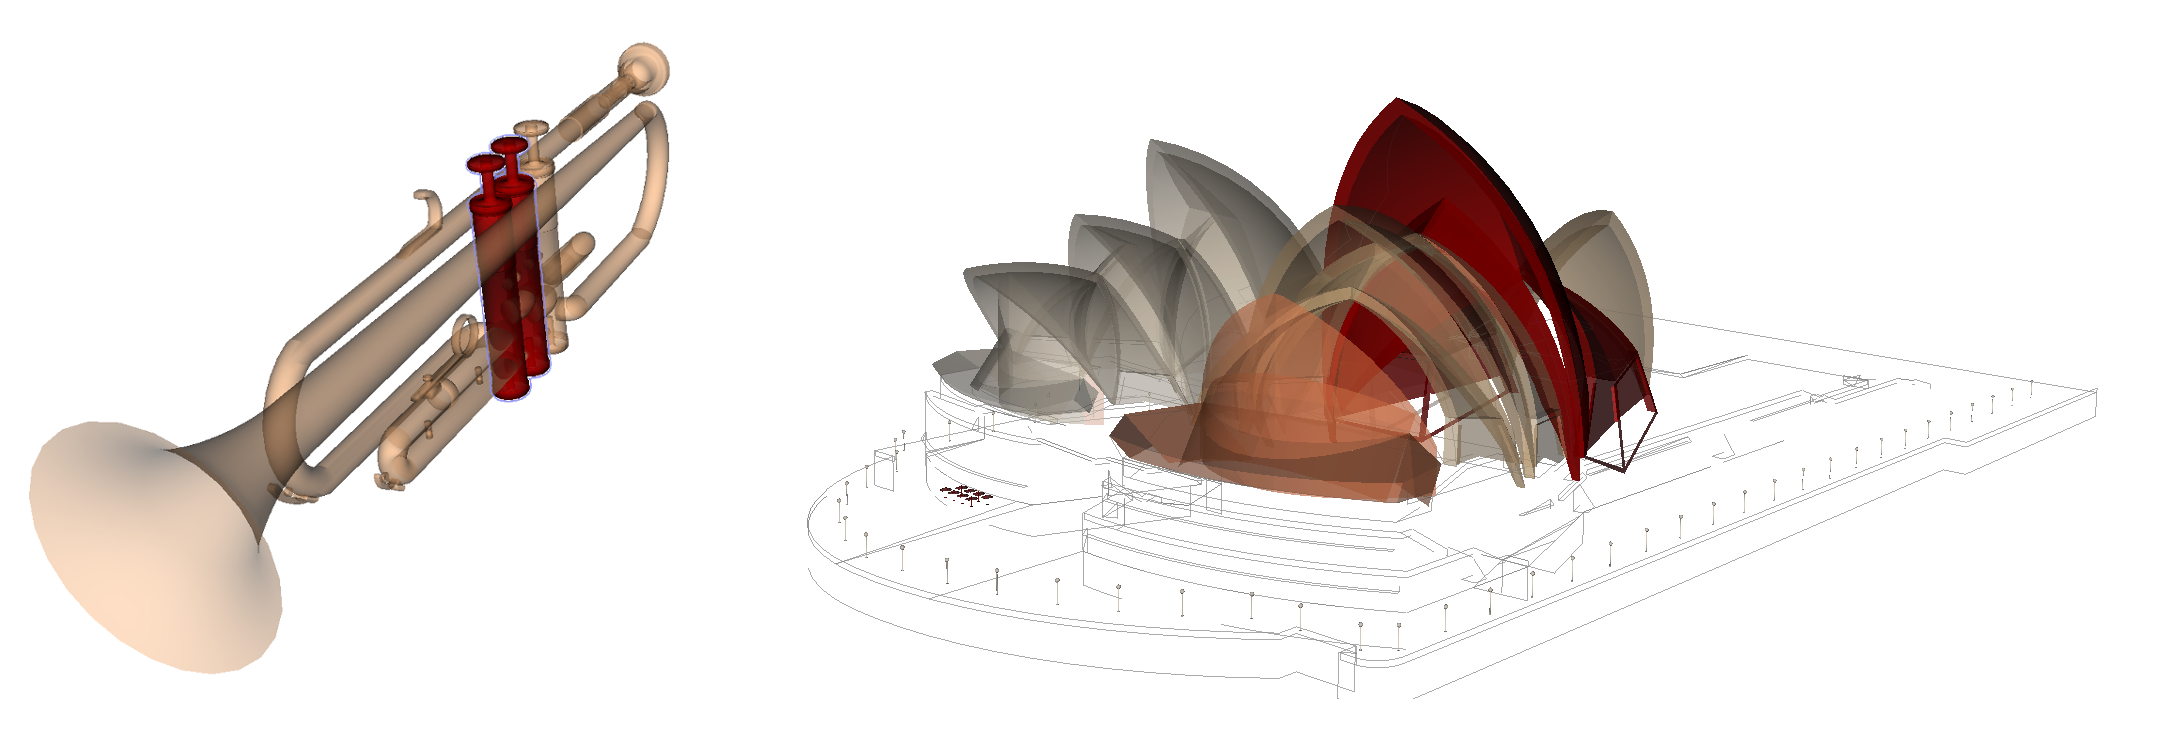
\includegraphics[width=\columnwidth]{future.png}  
	 \caption[Other Uses]{Possible usage for other domains: quality control for
	 musical instruments and building maintenance.}
	 \label{figure:future}
	\end{figure}
	% ============== 

Ambient settings is another possible area for future work, one can imaging using
camera planning algorithms to conduct a virtual tour of the entities while not
receiving input interactions. The said tour can be used to raise awareness of
particular features and highlight trends. The tour could be interrupted when a
person starts interacting with the display.

Lastly, while in this thesis we have primarily looked at the vehicle domain. Our
visualization approach is generalizable to other problems. Other analytical
tasks that relates text to physical productions may benefit from our approach. For
example see Figure \ref{figure:future}, where we show possible extensions
to look at quality control reports of a product such as a musical instrument,
and building maintenance records.


